%% This style is provided for the ICSE 2015 main conference,
%% ICSE 2015 co-located events, and ICSE 2015 workshops.

%% bare_conf_ICSE15.tex
%% V1.4
%% 2014/05/22


%% This is a skeleton file demonstrating the use of IEEEtran.cls
%% (requires IEEEtran.cls version 1.7 or later) with an IEEE conference paper.
%%
%% Support sites:
%% http://www.michaelshell.org/tex/ieeetran/
%% http://www.ctan.org/tex-archive/macros/latex/contrib/IEEEtran/
%% and
%% http://www.ieee.org/

%%*************************************************************************
%% Legal Notice:
%% This code is offered as-is without any warranty either expressed or
%% implied; without even the implied warranty of MERCHANTABILITY or
%% FITNESS FOR A PARTICULAR PURPOSE!
%% User assumes all risk.
%% In no event shall IEEE or any contributor to this code be liable for
%% any damages or losses, including, but not limited to, incidental,
%% consequential, or any other damages, resulting from the use or misuse
%% of any information contained here.
%%
%% All comments are the opinions of their respective authors and are not
%% necessarily endorsed by the IEEE.
%%
%% This work is distributed under the LaTeX Project Public License (LPPL)
%% ( http://www.latex-project.org/ ) version 1.3, and may be freely used,
%% distributed and modified. A copy of the LPPL, version 1.3, is included
%% in the base LaTeX documentation of all distributions of LaTeX released
%% 2003/12/01 or later.
%% Retain all contribution notices and credits.
%% ** Modified files should be clearly indicated as such, including  **
%% ** renaming them and changing author support contact information. **
%%
%% File list of work: IEEEtran.cls, IEEEtran_HOWTO.pdf, bare_adv.tex,
%%                    bare_conf.tex, bare_jrnl.tex, bare_jrnl_compsoc.tex
%%*************************************************************************

% *** Authors should verify (and, if needed, correct) their LaTeX system  ***
% *** with the testflow diagnostic prior to trusting their LaTeX platform ***
% *** with production work. IEEE's font choices can trigger bugs that do  ***
% *** not appear when using other class files.                            ***
% The testflow support page is at:
% http://www.michaelshell.org/tex/testflow/



% Note that the a4paper option is mainly intended so that authors in
% countries using A4 can easily print to A4 and see how their papers will
% look in print - the typesetting of the document will not typically be
% affected with changes in paper size (but the bottom and side margins will).
% Use the testflow package mentioned above to verify correct handling of
% both paper sizes by the user's LaTeX system.
%
% Also note that the "draftcls" or "draftclsnofoot", not "draft", option
% should be used if it is desired that the figures are to be displayed in
% draft mode.
%
\documentclass[conference]{IEEEtran}
%
\usepackage{url}

% If IEEEtran.cls has not been installed into the LaTeX system files,
% manually specify the path to it like:
% \documentclass[conference]{../sty/IEEEtran}





% Some very useful LaTeX packages include:
% (uncomment the ones you want to load)


% *** MISC UTILITY PACKAGES ***
%
%\usepackage{ifpdf}
% Heiko Oberdiek's ifpdf.sty is very useful if you need conditional
% compilation based on whether the output is pdf or dvi.
% usage:
% \ifpdf
%   % pdf code
% \else
%   % dvi code
% \fi
% The latest version of ifpdf.sty can be obtained from:
% http://www.ctan.org/tex-archive/macros/latex/contrib/oberdiek/
% Also, note that IEEEtran.cls V1.7 and later provides a builtin
% \ifCLASSINFOpdf conditional that works the same way.
% When switching from latex to pdflatex and vice-versa, the compiler may
% have to be run twice to clear warning/error messages.






% *** CITATION PACKAGES ***
%
%\usepackage{cite}
% cite.sty was written by Donald Arseneau
% V1.6 and later of IEEEtran pre-defines the format of the cite.sty package
% \cite{} output to follow that of IEEE. Loading the cite package will
% result in citation numbers being automatically sorted and properly
% "compressed/ranged". e.g., [1], [9], [2], [7], [5], [6] without using
% cite.sty will become [1], [2], [5]--[7], [9] using cite.sty. cite.sty's
% \cite will automatically add leading space, if needed. Use cite.sty's
% noadjust option (cite.sty V3.8 and later) if you want to turn this off.
% cite.sty is already installed on most LaTeX systems. Be sure and use
% version 4.0 (2003-05-27) and later if using hyperref.sty. cite.sty does
% not currently provide for hyperlinked citations.
% The latest version can be obtained at:
% http://www.ctan.org/tex-archive/macros/latex/contrib/cite/
% The documentation is contained in the cite.sty file itself.






% *** GRAPHICS RELATED PACKAGES ***
%
\ifCLASSINFOpdf
  \usepackage[pdftex]{graphicx}
  % declare the path(s) where your graphic files are
  % \graphicspath{{../pdf/}{../jpeg/}}
  % and their extensions so you won't have to specify these with
  % every instance of \includegraphics
  % \DeclareGraphicsExtensions{.pdf,.jpeg,.png}
\else
  % or other class option (dvipsone, dvipdf, if not using dvips). graphicx
  % will default to the driver specified in the system graphics.cfg if no
  % driver is specified.
  % \usepackage[dvips]{graphicx}
  % declare the path(s) where your graphic files are
  % \graphicspath{{../eps/}}
  % and their extensions so you won't have to specify these with
  % every instance of \includegraphics
  % \DeclareGraphicsExtensions{.eps}
\fi
% graphicx was written by David Carlisle and Sebastian Rahtz. It is
% required if you want graphics, photos, etc. graphicx.sty is already
% installed on most LaTeX systems. The latest version and documentation can
% be obtained at:
% http://www.ctan.org/tex-archive/macros/latex/required/graphics/
% Another good source of documentation is "Using Imported Graphics in
% LaTeX2e" by Keith Reckdahl which can be found as epslatex.ps or
% epslatex.pdf at: http://www.ctan.org/tex-archive/info/
%
% latex, and pdflatex in dvi mode, support graphics in encapsulated
% postscript (.eps) format. pdflatex in pdf mode supports graphics
% in .pdf, .jpeg, .png and .mps (metapost) formats. Users should ensure
% that all non-photo figures use a vector format (.eps, .pdf, .mps) and
% not a bitmapped formats (.jpeg, .png). IEEE frowns on bitmapped formats
% which can result in "jaggedy"/blurry rendering of lines and letters as
% well as large increases in file sizes.
%
% You can find documentation about the pdfTeX application at:
% http://www.tug.org/applications/pdftex





% *** MATH PACKAGES ***
%
%\usepackage[cmex10]{amsmath}
% A popular package from the American Mathematical Society that provides
% many useful and powerful commands for dealing with mathematics. If using
% it, be sure to load this package with the cmex10 option to ensure that
% only type 1 fonts will utilized at all point sizes. Without this option,
% it is possible that some math symbols, particularly those within
% footnotes, will be rendered in bitmap form which will result in a
% document that can not be IEEE Xplore compliant!
%
% Also, note that the amsmath package sets \interdisplaylinepenalty to 10000
% thus preventing page breaks from occurring within multiline equations. Use:
%\interdisplaylinepenalty=2500
% after loading amsmath to restore such page breaks as IEEEtran.cls normally
% does. amsmath.sty is already installed on most LaTeX systems. The latest
% version and documentation can be obtained at:
% http://www.ctan.org/tex-archive/macros/latex/required/amslatex/math/





% *** SPECIALIZED LIST PACKAGES ***
%
\usepackage{algpseudocode}
% algorithmic.sty was written by Peter Williams and Rogerio Brito.
% This package provides an algorithmic environment fo describing algorithms.
% You can use the algorithmic environment in-text or within a figure
% environment to provide for a floating algorithm. Do NOT use the algorithm
% floating environment provided by algorithm.sty (by the same authors) or
% algorithm2e.sty (by Christophe Fiorio) as IEEE does not use dedicated
% algorithm float types and packages that provide these will not provide
% correct IEEE style captions. The latest version and documentation of
% algorithmic.sty can be obtained at:
% http://www.ctan.org/tex-archive/macros/latex/contrib/algorithms/
% There is also a support site at:
% http://algorithms.berlios.de/index.html
% Also of interest may be the (relatively newer and more customizable)
% algorithmicx.sty package by Szasz Janos:
% http://www.ctan.org/tex-archive/macros/latex/contrib/algorithmicx/




% *** ALIGNMENT PACKAGES ***
%
%\usepackage{array}
% Frank Mittelbach's and David Carlisle's array.sty patches and improves
% the standard LaTeX2e array and tabular environments to provide better
% appearance and additional user controls. As the default LaTeX2e table
% generation code is lacking to the point of almost being broken with
% respect to the quality of the end results, all users are strongly
% advised to use an enhanced (at the very least that provided by array.sty)
% set of table tools. array.sty is already installed on most systems. The
% latest version and documentation can be obtained at:
% http://www.ctan.org/tex-archive/macros/latex/required/tools/


%\usepackage{mdwmath}
%\usepackage{mdwtab}
% Also highly recommended is Mark Wooding's extremely powerful MDW tools,
% especially mdwmath.sty and mdwtab.sty which are used to format equations
% and tables, respectively. The MDWtools set is already installed on most
% LaTeX systems. The lastest version and documentation is available at:
% http://www.ctan.org/tex-archive/macros/latex/contrib/mdwtools/


% IEEEtran contains the IEEEeqnarray family of commands that can be used to
% generate multiline equations as well as matrices, tables, etc., of high
% quality.


%\usepackage{eqparbox}
% Also of notable interest is Scott Pakin's eqparbox package for creating
% (automatically sized) equal width boxes - aka "natural width parboxes".
% Available at:
% http://www.ctan.org/tex-archive/macros/latex/contrib/eqparbox/





% *** SUBFIGURE PACKAGES ***
%\usepackage[tight,footnotesize]{subfigure}
% subfigure.sty was written by Steven Douglas Cochran. This package makes it
% easy to put subfigures in your figures. e.g., "Figure 1a and 1b". For IEEE
% work, it is a good idea to load it with the tight package option to reduce
% the amount of white space around the subfigures. subfigure.sty is already
% installed on most LaTeX systems. The latest version and documentation can
% be obtained at:
% http://www.ctan.org/tex-archive/obsolete/macros/latex/contrib/subfigure/
% subfigure.sty has been superceeded by subfig.sty.



%\usepackage[caption=false]{caption}
%\usepackage[font=footnotesize]{subfig}
% subfig.sty, also written by Steven Douglas Cochran, is the modern
% replacement for subfigure.sty. However, subfig.sty requires and
% automatically loads Axel Sommerfeldt's caption.sty which will override
% IEEEtran.cls handling of captions and this will result in nonIEEE style
% figure/table captions. To prevent this problem, be sure and preload
% caption.sty with its "caption=false" package option. This is will preserve
% IEEEtran.cls handing of captions. Version 1.3 (2005/06/28) and later
% (recommended due to many improvements over 1.2) of subfig.sty supports
% the caption=false option directly:
%\usepackage[caption=false,font=footnotesize]{subfig}
%
% The latest version and documentation can be obtained at:
% http://www.ctan.org/tex-archive/macros/latex/contrib/subfig/
% The latest version and documentation of caption.sty can be obtained at:
% http://www.ctan.org/tex-archive/macros/latex/contrib/caption/




% *** FLOAT PACKAGES ***
%
%\usepackage{fixltx2e}
% fixltx2e, the successor to the earlier fix2col.sty, was written by
% Frank Mittelbach and David Carlisle. This package corrects a few problems
% in the LaTeX2e kernel, the most notable of which is that in current
% LaTeX2e releases, the ordering of single and double column floats is not
% guaranteed to be preserved. Thus, an unpatched LaTeX2e can allow a
% single column figure to be placed prior to an earlier double column
% figure. The latest version and documentation can be found at:
% http://www.ctan.org/tex-archive/macros/latex/base/



%\usepackage{stfloats}
% stfloats.sty was written by Sigitas Tolusis. This package gives LaTeX2e
% the ability to do double column floats at the bottom of the page as well
% as the top. (e.g., "\begin{figure*}[!b]" is not normally possible in
% LaTeX2e). It also provides a command:
%\fnbelowfloat
% to enable the placement of footnotes below bottom floats (the standard
% LaTeX2e kernel puts them above bottom floats). This is an invasive package
% which rewrites many portions of the LaTeX2e float routines. It may not work
% with other packages that modify the LaTeX2e float routines. The latest
% version and documentation can be obtained at:
% http://www.ctan.org/tex-archive/macros/latex/contrib/sttools/
% Documentation is contained in the stfloats.sty comments as well as in the
% presfull.pdf file. Do not use the stfloats baselinefloat ability as IEEE
% does not allow \baselineskip to stretch. Authors submitting work to the
% IEEE should note that IEEE rarely uses double column equations and
% that authors should try to avoid such use. Do not be tempted to use the
% cuted.sty or midfloat.sty packages (also by Sigitas Tolusis) as IEEE does
% not format its papers in such ways.





% *** PDF, URL AND HYPERLINK PACKAGES ***
%
%\usepackage{url}
% url.sty was written by Donald Arseneau. It provides better support for
% handling and breaking URLs. url.sty is already installed on most LaTeX
% systems. The latest version can be obtained at:
% http://www.ctan.org/tex-archive/macros/latex/contrib/misc/
% Read the url.sty source comments for usage information. Basically,
% \url{my_url_here}.


\usepackage{tikz}
\usepackage{booktabs}


% *** Do not adjust lengths that control margins, column widths, etc. ***
% *** Do not use packages that alter fonts (such as pslatex).         ***
% There should be no need to do such things with IEEEtran.cls V1.6 and later.
% (Unless specifically asked to do so by the journal or conference you plan
% to submit to, of course. )


% correct bad hyphenation here
\hyphenation{op-tical net-works semi-conduc-tor}


\begin{document}
%
% paper title
% can use linebreaks \\ within to get better formatting as desired
\title{Drawing Representative Conclusions about Software: A Sampling Technique and New Spreadsheet Corpus}


% author names and affiliations
% use a multiple column layout for up to three different
% affiliations
%\author{\IEEEauthorblockN{Michael Shell}
%\IEEEauthorblockA{School of Electrical and\\Computer Engineering\\
%Georgia Institute of Technology\\
%Atlanta, Georgia 30332--0250\\
%Email: http://www.michaelshell.org/contact.html}
%\and
%\IEEEauthorblockN{Homer Simpson}
%\IEEEauthorblockA{Twentieth Century Fox\\
%Springfield, USA\\
%Email: homer@thesimpsons.com}
%\and
%\IEEEauthorblockN{James Kirk\\ and Montgomery Scott}
%\IEEEauthorblockA{Starfleet Academy\\
%San Francisco, California 96678-2391\\
%Telephone: (800) 555--1212\\
%Fax: (888) 555--1212}}

% conference papers do not typically use \thanks and this command
% is locked out in conference mode. If really needed, such as for
% the acknowledgment of grants, issue a \IEEEoverridecommandlockouts
% after \documentclass

% for over three affiliations, or if they all won't fit within the width
% of the page, use this alternative format:
%
\author{\IEEEauthorblockN{Titus Barik\IEEEauthorrefmark{1},
John Slankas\IEEEauthorrefmark{1},
Kevin Lubick\IEEEauthorrefmark{1},
Felienne Hermans\IEEEauthorrefmark{2} and
Emerson Murphy-Hill\IEEEauthorrefmark{1}}
\IEEEauthorblockA{\IEEEauthorrefmark{1}North Carolina State University, USA\\
\{tbarik, john.slankas, kjlubick\}@ncsu.edu, emerson@csc.ncsu.edu}
\IEEEauthorblockA{\IEEEauthorrefmark{2}Delft University of Technology, Netherlands\\f.f.j.hermans@tudelft.nl}}




% use for special paper notices
%\IEEEspecialpapernotice{(Invited Paper)}




% make the title area
\maketitle


\begin{abstract}
Spreadsheets users are the largest group of software developers on
the planet, and much of what researchers know about this group derives
from the EUSES corpus, a corpus that includes about 5,000 spreadsheets
mined from the web a decade ago.
While the EUSES corpus has yielded many interesting research results,
the corpus is aging and small, relative to the number of spreadsheets
used today.
Moreover, the EUSES corpus was obtained entirely from spreadsheets posted
to the public web.
In this paper, we introduce several new spreadsheet corpora: one corpus contains
about 1.5 million open-source spreadsheets mined from the public web, 
and three others mined from formerly closed-source email attachments from the Stratfor intelligence
company, the Enron energy firm, and the Syrian government.
We also use these corpora to introduce a new sampling techinque that allows researchers to 
create their own open-source software corpus that is representative of 
a a closed-source corpus.
We evaluate the utility of our technique by 
replicating part of a recent spreadsheet study and showing
how results from subsampled open-source are equivalent to 
results obtained from the original closed-source corpus.
%TODO add some interesting results
\end{abstract}
% IEEEtran.cls defaults to using nonbold math in the Abstract.
% This preserves the distinction between vectors and scalars. However,
% if the conference you are submitting to favors bold math in the abstract,
% then you can use LaTeX's standard command \boldmath at the very start
% of the abstract to achieve this. Many IEEE journals/conferences frown on
% math in the abstract anyway.

% no keywords




% For peer review papers, you can put extra information on the cover
% page as needed:
% \ifCLASSOPTIONpeerreview
% \begin{center} \bfseries EDICS Category: 3-BBND \end{center}
% \fi
%
% For peerreview papers, this IEEEtran command inserts a page break and
% creates the second title. It will be ignored for other modes.
\IEEEpeerreviewmaketitle

\section{Introduction}

Spreadsheets are an important type of software that is developed today.
Scaffidi and colleagues estimate that there are more than 55 million end user
spreadsheet or database users in the US alone~\cite{scaffidi2005estimating}.

Underscoring how spreadsheet development is a specific area of the more general
area of software development,
bugs in spreadsheets have resulted in substantial losses, economic and otherwise.
For example, Reinhart and Rogoff reported on their analysis of data in Excel in 
a working paper that concluded that countries with high economic debt-to-GDP
ratios have slow economic growth~\cite{reinhart2010growth}.
Powerful politicians have used this result to implement debt-reducing measures
across Europe, in an attempt to increase economic growth~\cite{cassidy}.
However, after the original spreadsheet was shared with scientists doing a replication
study, it was revealed that the original spreadsheet contained a selection error,
which reversed the paper's main findings about debt and growth~\cite{coy}.

As a consequence of the importance of spreadsheets, significant existing research
has studied spreadsheets in a variety of contexts.
For example, at ICSE 2007, Abraham and Erwig evaluated GoalDebug, a spreadsheet
debugger~\cite{abraham2007goaldebug}; at ICSE 2012; Hermans and colleagues presented a method for
detecting and visualizating spreadsheet smells~\cite{hermans2012detecting}; and 
at ICSE 2014, Dou and colleagues presented AmCheck,
a tool that finds and repairs ambiguous computations~\cite{dou2014spreadsheet}.
%TODO we need to drive home spreadsheet stuff appeasr at ICSE if a non-spreadsheet person gets the paper

A significant amout of prior work on spreadsheets does formative or evaluative 
studies using the EUSES corpus, a set of 4,498 spreadsheets published in 2005.
Abraham and Erwig use the EUSES corpus to motivate their approach~\cite{abraham2007goaldebug};
Hermans and colleagues used EUSES to set thresholds 
for their code smells~\cite{hermans2012detecting}; and Dou and colleagues
use EUSES to determine how often ambiguous computation occurs~\cite{dou2014spreadsheet}.

% TODO has someone else raised public concerns about the representtaiveness of EUSES?
% Currently, the most used corpus for spreadsheet analysis is the EUSES corpus.
% This corpus contains spreadsheets obtained mainly by searching in search
% engines, so it contains spreadsheets that are publicly available. However,
% industrial case studies performed by us and other researchers have raised
% questions about the representativeness of this corpus~\cite{something}, as spreadsheets we 
% encounter in industry tend to be bigger and be more complex. Hence, we believe
% there is a need for a corpus providing a more realistic test set for spreadsheet
% researchers.

In this paper, we introduce several new spreadsheet corpora.
Why do we need more spreadsheet corpora, beyond EUSES, which has served the community so well?
\begin{itemize}
  \item
  	Although EUSES is the largest spreadsheet corpus today, it is relatively small by
  	modern software repository standards; EUSES has about 4.5 thousand spreadsheets, while 
  	Sourceforge lists 350 thousand software projects\footnote{\url{http://sourceforge.net/blog/sourceforge-myths/}} 
  	and OpenHub lists about 666 thousand
  	software projects.\footnote{\url{https://www.openhub.net/explore/projects}}
  \item
  	Most EUSES spreadsheets were obtained through the public world-wide-web,
  	what we might call \emph{open source} spreadsheets; the remaining 97 spreadsheets were obtained
  	largely from textbook examples. What is missing is a substantial set of \emph{closed source} spreadsheets, that is,
  	spreadsheets that were not intended to be made available to the public.
  \item
  	The EUSES corpus is not publicly available. To use it, ``you must be a researcher in the field of 
  	software engineering, end-user programming, human-computer interaction, or 
  	usability'',\footnote{\url{http://eusesconsortium.org/resources.php}} 
  	and even then, the researcher must explicitly ask for a copy by email.
  \item
  	The EUSES corpus is about a decade old, leaving out a large number of recently
  	created spreadsheets.
  	%TODO probably want to know something about the dates, if you're claiming you're newer
\end{itemize}

In this paper we also introduce a new technique and associated tool designed to enable researchers 
to create subsamples of a software corpus such that the subsample approximates 
another corpus.
This is useful in situations where a research group has access to a private software
corpus that they cannot pubically release, but can instead release a corpus profile
that enables other researchers to run their analysis on a simulation of the private corpus.
For example, in the context of spreadsheets, if a research group has access to 
a private corpus of healthcare spreadsheets, they can extract and share a corpus profile
with other researchers, who can then use our spreadsheet corpora and the extracted profile to create
a new public subsample that approximates the private corpus.

The contributions of this paper are:

\begin{itemize}
  \item An open-source corpus of spreadsheets more than two orders of magnitude larger
 		than the existing state of the art,;
  \item Three never-before analyzed, formerly closed-source corpora of spreadsheets extracted
  		from private email exchanges made public by Wikileaks and the United States Federal 
  		Energy Regulatory Commission;
  		%TODO each larger than EUSES?
  \item A new technique for creating representative subsamples of open-source
  		software; and
  %TODO the following is bonus, if we can
  %\item A set of distributions of real closed-source spreadsheets that can be
  %		used as parameters to our technique; and
  \item An evaluation that demonstrates 
		how research results on a corpus obtained using our subsampling technique
		are similar to results obtained from a target corpus.
\end{itemize}

\section{Prior Work}

Maybe a bit more depth in spreadsheet research, showing how serious it is.

A good bit from Mei Nagappan's representativeness paper~\cite{nagappan2013diversity}.

Based on that sampling thing represented by the stats professor,
though that's not a technique.

\section{Our Technique}

The aim of our sampling technique is to take a corpus of software, be it 
a collection of Excel spreadsheets, open source projects on Github, 
or some other software, and extract a subset of that corpus that represents
some other corpus.
The former we will call the ``subsampled corpus'', and the latter the
``target corpus.''

The reason we want a corpus to approximate a target corpus is because the 
target may be unavailable for analysis.
For example, suppose that we wanted to do an anaysis of financial spreadsheets,
but we had no open-source financial spreadsheets available.
Suppose further that we do know several financial firms that have such spreadsheets,
but (a) they cannot legally share those spreadsheets with us, and (b) if we somehow wrote a paper
about those spreadsheets, we would be unable to share the spreadsheets with other researchers
to enable future replications.

Thus, we designed our technique to extract a subsampled corpus that \emph{represents}
the target corpus.
In our example, the target corpus is the closed-source set of spreadsheets that the 
financial firms has.
The corpus from which we draw our subsample should be some large, existing corpus, such
as the existing EUSES corpus or our open-source corpus introduced in this paper.

%TODO maybe ``subsample'' should be ``subcorpus''?

Prior to our technique, drawing a representative subsample of software was largely
informal.
In the case of the EUSES corpus, an expicitly labeled subsample is identified as ``financial spreadsheets'',
which were identified as such because the Google search for this subsample
contained the word ``financial.''
However, it is possible that some spreadsheets that could be categorized as financial do not
use the word ``financial,'' and that some spreadsheets that do contain that keyword might not
actually be financial at all.
Analagously, in prior work we've shown that explicit labels are poor indicators of developers'
activities; in the domain of refactoring, commits containing refactoring keywords are \emph{less}
likely to contain refactoring code transformations than commits without those keywords~\cite{HowWeRefactor}.

%TODO more subsections, so this is easier to skim

Informally, our technique works as follows.
For each item (spreadsheet, software project, etc.) in a target corpus and each
item in a sample corpus, extract a vector of $n$ metrics from each item.
These metrics might be, for example, for spreadsheets, number of cells,
number of formulas, and number of worksheets.
Then, given the number of items we desire in our subsampled corpus,
we select that many items from our sample corpus such that
the set of metric vectors in the subsample approximates thet set
of metric vectors in the target corpus.

In the remainder of this section, we describe Nagappan and colleagues'
diversity algorithm, on which our technqiue is based; 
a more technical description of technique and our R-based implementation;
and limitations of our approach.

\subsection{Nagappan's Diversity Algorithm}

\begin{figure}[!t]
\begin{algorithmic}
\If {$i\geq maxval$}
    \State $i\gets 0$
\Else
    \If {$i+k\leq maxval$}
        \State $i\gets i+k$
    \EndIf
\EndIf
\end{algorithmic}
\caption{A sample algorithm.}
\label{fig:algorithm}
\end{figure}

It's like theirs~\cite{nagappan2013diversity}.

\subsection{Our Technique and Implementation}

\subsection{Limitations}

Obviously, only as good as our metrics. Implies correlation. Counterexample: color.
This is kind of what we do intutively anyway, when we say we chose large, mature projects -- we intend them
to be representative.

You need a good corpus to sample from.

\section{The Corpora}

In this section, we describe our corpora of spreadsheets
and how we obtained them.
A summary of the spreadsheets is shown in Table~\ref{tab:corpusoverview}.

\begin{table}
	\caption{A summary of the state of the art corpus, \textit{in italics},
	and our corpora.}\label{tab:corpusoverview}
	
	\begin{tabular}{ l r r }
		\toprule
		\textbf{Corpus} & \textbf{Number of Spreadsheets} & \textbf{Size of Corpus}\\
		\midrule	  	
	  	\textit{EUSES~\cite{fisher2005euses}} & \textit{4,498} & \textit{? GB}\\	  	
	  	Open Source & 1,534,669 & 890.? GB \\
	  	Enron & 11,985 & ? GB \\ 
		Stratfor & 10,529 & 2.3 GB\\
		Syria & 2,633 & 0.2 GB\\
		%TODO fill in missing values
		\bottomrule
	\end{tabular}
\end{table}

\subsection{The Open-Source Corpus}



% URLs from original Dremel query: 1,626,610
% Excel spreadsheets downloaded from EC2: 1,534,669
% Size of spreadsheets downloaded from EC2: TODO(tbarik)

We obtained the Excel spreadsheets for this corpus through a proprietary, corporate index of public world wide web documents from July 16, 2014. 
%
Each document object within the index contains a canonical URL, and reasonable efforts, such as duplication elimination, are made so that each object points to unique content. 
%
From this index, we extracted the canonical URLs for which the document format was tagged as \texttt{application/vnd.ms-excel}, that is, a Microsoft Excel spreadsheet. 
%
From this process, we obtained approximately 1.6 million spreadsheet URLs.

We then fed these URLs into a download script, discarding URLs that returned an invalid status code (such as \texttt{404: Not Found}), URLs that referenced FTP content (URLs beginning with \texttt{ftp://}), and URLs whose download failed to complete within 60 seconds on a 100 MB/s network link. 
%
We re-ran the script for failed URLs after a 24 our period, to account for sites that may have been temporarily down. 
%
In total, we downloaded 1.5 million Microsoft Excel spreadsheets (820 GB). 

%TODO where can the reader download the files?

\subsection{The Enron Corpus}

While our Open Source corpus provides a larger data set than the EUSES corpus, 
it likely still misses the context of closed-source spreadsheets. 
Therefore we present a second data set in the paper, derived from
the Enron E-mail Archive.\footnote{\url{https://www.cs.cmu.edu/~./enron/}} 
This is an large database of 619,446 emails
containing emails from by 158 Enron employees~\cite{klimt2004introducing}.
The email dataset was originally released by the United States 
Federal Energy Regulatory Commission, and contain emails from the 
late 1990s to the early 2000s in the wake the bankrupcy of the Enron
energy corporation~\cite{grieve}.

We first requested the most recent version of the dataset, 
version 1.3, last updated July 29 , 2013. This version contains 130
folders with 190 Micrsoft Outlook data files, and is 53 gigabytes in size.
Using the SysTools' Outlook Attachment 
Extractor,\footnote{\url{http://www.systoolsgroup.com/outlook-attachment-extractor.html}} 
we extracted the spreadsheets from the Outlook data files. 
%With the extractor, obtaining all spreadsheets took
%about 6 hours, on an i7 machine with 16 gig memory. 
In total, the email data set
contains 265,586 files (32.3 gigs), of which over 50,000 are Excel spreadsheets. 
Using MD5 hashes to find and remove duplicates spreadsheet files,
we are left with 16,188 unique spreadsheets.

\subsection{The Stratfor Corpus}

In 2012, Wikileaks published more than 5 million private emails from the
intelligence company Stratfor.\footnote{\url{https://wikileaks.org/the-gifiles.html}}
While the dataset contained emails from 2000 to 2012, 
the year with the most emails was 2011.
From this dataset, we extracted 10,529 
unique Excel files, about 2.25 gigabytes in total.

\subsection{The Syrian Corpus}

In 2012, Wikileaks pushed more than 2 million private emails from
the Syrian government and affiliated companies.\footnote{\url{https://wikileaks.org/syria-files/}}
While the dataset contains emails from 2006 through 2012, 
the year with the most emails was 2012.
From this dataset, we extracted 2,633 spreadsheets, about 227 megabytes in total.

\subsection{Corpora Characterization}

Compare the spreadsheet sets to each other.

Number of spreadsheets, a few stats about them.

Distribution comparison to EUSES here?

From Enron:

\section{Analysis of the Spreadsheets}
For all the spreadsheets, we ran the Spreadsheet Scantool, developed at Delft University of Technology. This tool runs on the previously developed Breviz core, made for spreadsheet visualization and smell detection. TODO: References. 14,579 spreadsheets could be analyzed, the others were password protected, corrupt, or otherwise unreadable.

\subsection{Files}
In total, our set of analyzable spreadsheets contains of 14,579 files. Their average file size is TODO.

\subsection{Worksheets}
In total the 14,579 spreadsheets contain 51,015 worksheets, which is an average of 4,6 worksheets per spreadsheet. The spreadsheet with the most worksheets has no less than 96 worksheets. The following graph shows the distribution of worksheets over the spreadsheets.

\begin{figure}[ht!]
\centering
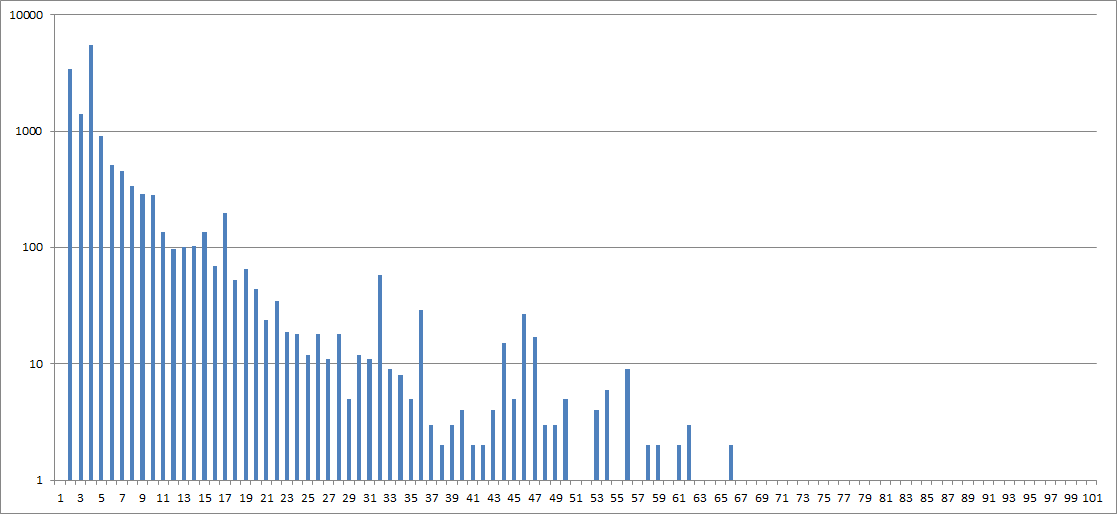
\includegraphics[width=90mm]{Worksheets.png}
\caption{Distribution of number of worksheets over the spreadsheet files.}
\label{overflow}
\end{figure}

\subsection{Cells}
The 14,579 spreadsheets together have 102,919,261 non-empty cells of which 6,684,233 are formulas.

\subsection{Formulas}
Not all spreadsheets in the Enron set contain formulas: there are ... files containing formulas, which is about half of all spreadsheets in the set. Note this ratio is a lot higher than that of the EUSES corpus, which contains ... spreadsheets but only 1711 with formulas.

Together the ... files with formulas contain ... formulas and ... unique formulas. This means the average spreadsheet \emph{with formulas} contains ... of them.



\begin{figure}[!t]
\centering
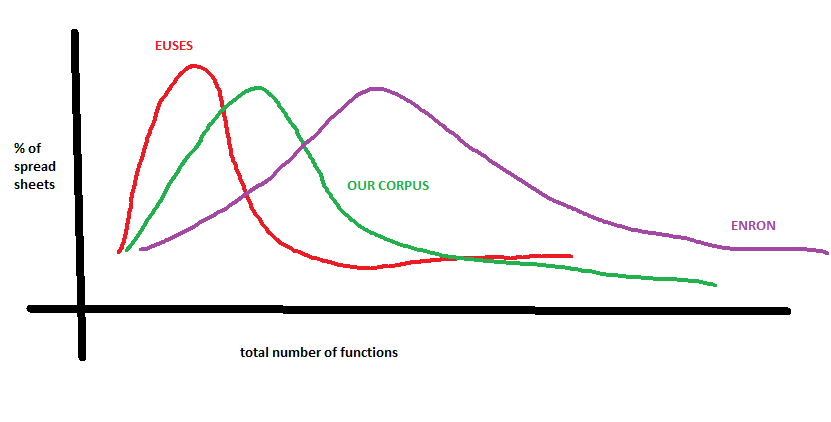
\includegraphics[width=\columnwidth]{functions.png}
\caption{Distribution of number of fuctions per spreadsheet, for 3 spreadsheet corpuses.}
\label{fig:functions}
\end{figure}

\section{Distributions from Real Closed-Source Code}

Describe dataset.
Talk about distribution. (plot distribution on same axis, maybe three different metrics).

\section{Evaluation}

RQ1: Do the conclusions from existing studies change depending on what corpus they use? (Compare uses to others)
RQ2: Do conclusions drawn using our sampling technique approximate conclusions from original sample?

The study we replicate is an evaluation of Barowy, Gochev, and Berger's
CheckCell tool~\cite{barowy14}, a tool that was built to identify spreadsheet
cells that have an inordanately high impact on calculations.
The intuition is that such cells may contain data input errors.

As part of their evaluation, CheckCell's authors wanted to know whether checkcell runs efficiently
To evaluate efficiency, the authors randomly selected 64 spreadsheets that contained at least one
formula from the EUSES corpus, then ran their analysis on a commodity laptop.
They conclude, ``For most of the spreadsheets, CheckCell completes its analysis in under 50 seconds;
for all but two, it completes in under five minutes.''
The results for all spreadsheets are shown as blue bars on Figure~\ref{fig:effectiveness}.

%TODO Titus wants to do more than just time -- wants to detect errors.

\begin{figure}[!t]
\centering
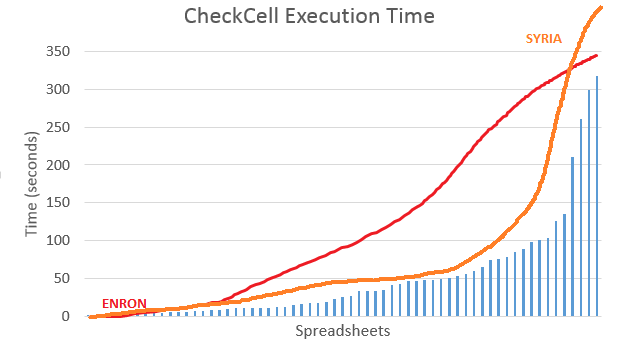
\includegraphics[width=\columnwidth]{checkcell.png}
\caption{CheckCell efficiency data.}
\label{fig:effectiveness}
\end{figure}

We first used our VCL infrastructure to run CheckCell on all EUSES spreadsheets; we assume
that Borowy and colleagues did not do this originally for efficiency reasons.
We then ran the results on each of our other data sets.
The results are overlaid on Figure~\ref{fig:effectiveness}.
We then performed an unpaired t-test to determine whether there were significant differences
in the distributions.
%TODO probably want ot make sure distributions are normal first

The results suggest that:
- Outcome 1: No significant differences. Does this diminish the need for our technique?
  Perhaps we can say that our approach confirms that Bowory's sampling was reasonable,
  and that euses is a good 
- Outcome 2: No differences between open source sets, but some between open and closed. 
  Tells us that the closed ones are systematically different.
- Outcome 3: Differnece between open source sets. The most interesting! Says something about 
  sampling methods.


\section{Limitations}

Automation (VBA/Interop) vs. snapshot parsing. Can't know definitely when
something is an error.
%
Dependency analysis limitations.
%
Parsing function limitations.
%
Excel 95 spreadsheets not supported. Not a big problem though. EUSES corpus did have some of these. Trade-off between keeping files in Excel 97 and changing them to xlsx -- macros dissapear in the latter unless it is xlsm.
%
VBA analysis not supported until new security model.
%
What is an error? Move somewhere else: Cells containing formulas that result in an error. The error appears because the formula doesn't use the expected syntax, arguments, or data types. Error values include \texttt{\#\#\#\#\#}, \texttt{\#DIV/0!}, \texttt{\#N/A}, \texttt{\#NAME?}, \texttt{\#NULL!}, \texttt{\#NUM!}, \texttt{\#REF!}, and \texttt{\#VALUE!}. Each error value has different causes and is resolved in different ways. Also, change this text since it matches MSDN right now.

% http://www.gemboxsoftware.com/Spreadsheet/Help/html/P_GemBox_Spreadsheet_ExcelCell_Formula.htm
Old XLS format requires all formulas to be parsed and saved to XLS files as special tokens in RPN (Reverse Polish notation). GemBox.Spreadsheet only knows how to parse limited set of formulas listed below.

New XLSX (Open XML) format stores formulas as strings and leaves formula parsing to applications that read XLSX documents. Therefore, ALL formulas are supported when writing/reading XLSX files.

Other limitations to the study.

\section{Conclusions}



% An example of a floating figure using the graphicx package.
% Note that \label must occur AFTER (or within) \caption.
% For figures, \caption should occur after the \includegraphics.
% Note that IEEEtran v1.7 and later has special internal code that
% is designed to preserve the operation of \label within \caption
% even when the captionsoff option is in effect. However, because
% of issues like this, it may be the safest practice to put all your
% \label just after \caption rather than within \caption{}.
%
% Reminder: the "draftcls" or "draftclsnofoot", not "draft", class
% option should be used if it is desired that the figures are to be
% displayed while in draft mode.
%
%\begin{figure}[!t]
%\centering
%\includegraphics[width=2.5in]{myfigure}
% where an .eps filename suffix will be assumed under latex,
% and a .pdf suffix will be assumed for pdflatex; or what has been declared
% via \DeclareGraphicsExtensions.
%\caption{Simulation Results}
%\label{fig_sim}
%\end{figure}

% Note that IEEE typically puts floats only at the top, even when this
% results in a large percentage of a column being occupied by floats.


% An example of a double column floating figure using two subfigures.
% (The subfig.sty package must be loaded for this to work.)
% The subfigure \label commands are set within each subfloat command, the
% \label for the overall figure must come after \caption.
% \hfil must be used as a separator to get equal spacing.
% The subfigure.sty package works much the same way, except \subfigure is
% used instead of \subfloat.
%
%\begin{figure*}[!t]
%\centerline{\subfloat[Case I]\includegraphics[width=2.5in]{subfigcase1}%
%\label{fig_first_case}}
%\hfil
%\subfloat[Case II]{\includegraphics[width=2.5in]{subfigcase2}%
%\label{fig_second_case}}}
%\caption{Simulation results}
%\label{fig_sim}
%\end{figure*}
%
% Note that often IEEE papers with subfigures do not employ subfigure
% captions (using the optional argument to \subfloat), but instead will
% reference/describe all of them (a), (b), etc., within the main caption.


% An example of a floating table. Note that, for IEEE style tables, the
% \caption command should come BEFORE the table. Table text will default to
% \footnotesize as IEEE normally uses this smaller font for tables.
% The \label must come after \caption as always.
%
%\begin{table}[!t]
%% increase table row spacing, adjust to taste
%\renewcommand{\arraystretch}{1.3}
% if using array.sty, it might be a good idea to tweak the value of
% \extrarowheight as needed to properly center the text within the cells
%\caption{An Example of a Table}
%\label{table_example}
%\centering
%% Some packages, such as MDW tools, offer better commands for making tables
%% than the plain LaTeX2e tabular which is used here.
%\begin{tabular}{|c||c|}
%\hline
%One & Two\\
%\hline
%Three & Four\\
%\hline
%\end{tabular}
%\end{table}


% Note that IEEE does not put floats in the very first column - or typically
% anywhere on the first page for that matter. Also, in-text middle ("here")
% positioning is not used. Most IEEE journals/conferences use top floats
% exclusively. Note that, LaTeX2e, unlike IEEE journals/conferences, places
% footnotes above bottom floats. This can be corrected via the \fnbelowfloat
% command of the stfloats package.



\section{Conclusion}
The conclusion goes here.




% conference papers do not normally have an appendix


% use section* for acknowledgement
\section*{Acknowledgment}


The authors would like to thank...





% trigger a \newpage just before the given reference
% number - used to balance the columns on the last page
% adjust value as needed - may need to be readjusted if
% the document is modified later
%\IEEEtriggeratref{8}
% The "triggered" command can be changed if desired:
%\IEEEtriggercmd{\enlargethispage{-5in}}

% references section

% can use a bibliography generated by BibTeX as a .bbl file
% BibTeX documentation can be easily obtained at:
% http://www.ctan.org/tex-archive/biblio/bibtex/contrib/doc/
% The IEEEtran BibTeX style support page is at:
% http://www.michaelshell.org/tex/ieeetran/bibtex/
\bibliographystyle{IEEEtran}
% argument is your BibTeX string definitions and bibliography database(s)
\bibliography{IEEEabrv,references}

% that's all folks
\end{document}


